\documentclass[11pt]{article}
\usepackage{graphicx}
\DeclareGraphicsExtensions{.png,.jpg}
\graphicspath{{./figures/}}

\begin{document}

\title{Architecture of the Proposed Cloud Application Platform Monitor}
\author{Chandra Krintz, Rich Wolski, Hiranya Jayathilaka, Wei-Tsung Lin}
\maketitle

\section{Introduction}
Over the last decade Platform-as-a-Service (PaaS) has become a popular approach for deploying
applications in the cloud. Many organizations, academic institutes and hobbyists make use of public
and/or private PaaS clouds to deploy their applications.
PaaS clouds provide a high level of abstraction to the application developer that effectively hides
all the infrastructure-level details such as physical resource allocation (CPU, memory, disk etc), operating
system configuration, 
and network set up. This enables application developers to focus solely on the programming
aspects of their applications, without having to be concerned about deployment issues. PaaS
clouds can also ensure high levels of scalability and availability for the deployed applications. 
Scalability is typically provided by automatically allocating resources for applications
on the fly (auto scaling), and availability is ensured by running multiple instances of the application.
Consequently the viable PaaS technologies, and the PaaS-deployed applications
continue to increase in number.

This rapid growth in PaaS technology has intensified the need for new techniques to
monitor applications deployed in a PaaS cloud. Application developers and users wish
to monitor the availability of the deployed applications, track application performance and detect 
application and system anomalies as they occur. To obtain this level of deep operational insight into
PaaS-deployed applications, the PaaS clouds need to be equipped with powerful instrumentation,
data gathering and analysis capabilities that span the entire stack of the PaaS cloud. 
Moreover, PaaS clouds need to provide comprehensive
data visualization and notification mechanisms. However, most PaaS technologies available
today either do not provide any application monitoring support, or only provide primitive
monitoring features such as application-level logging. Hence, they are not capable of performing
powerful predictive analyses or anomaly detection, which require much more fine-grained, low-level
and full stack data collection and analytics. 

To address this limitation we intend to design and implement a comprehensive application platform 
monitor (APM) that can be easily integrated with a wide variety of PaaS technologies. The proposed
APM is not an external system that monitors a PaaS cloud from the outside. Rather, it integrates with
the PaaS cloud from within thereby extending and augmenting the existing components of the PaaS cloud
to provide comprehensive full stack monitoring, analytics and visualization capabilities. In other words,
the APM is built into the PaaS cloud so that it is active as long as the cloud is, and has operational
insight to both core cloud components as well as the deployed applications.

This document details the architecture of the proposed APM, and how it integrates with a typical PaaS
cloud. We describe individual components of the APM, their functions and how they interact with each
other. Where appropriate we also detail the concrete technologies (tools and products) used to implement
various components of the APM, and give rationale for choosing those technologies.

We start by describing the layered system organization typically seen in PaaS clouds. Then we describe
the APM architecture, and show how it fits into the PaaS.

\section{PaaS System Organization}
\begin{figure}
\centering
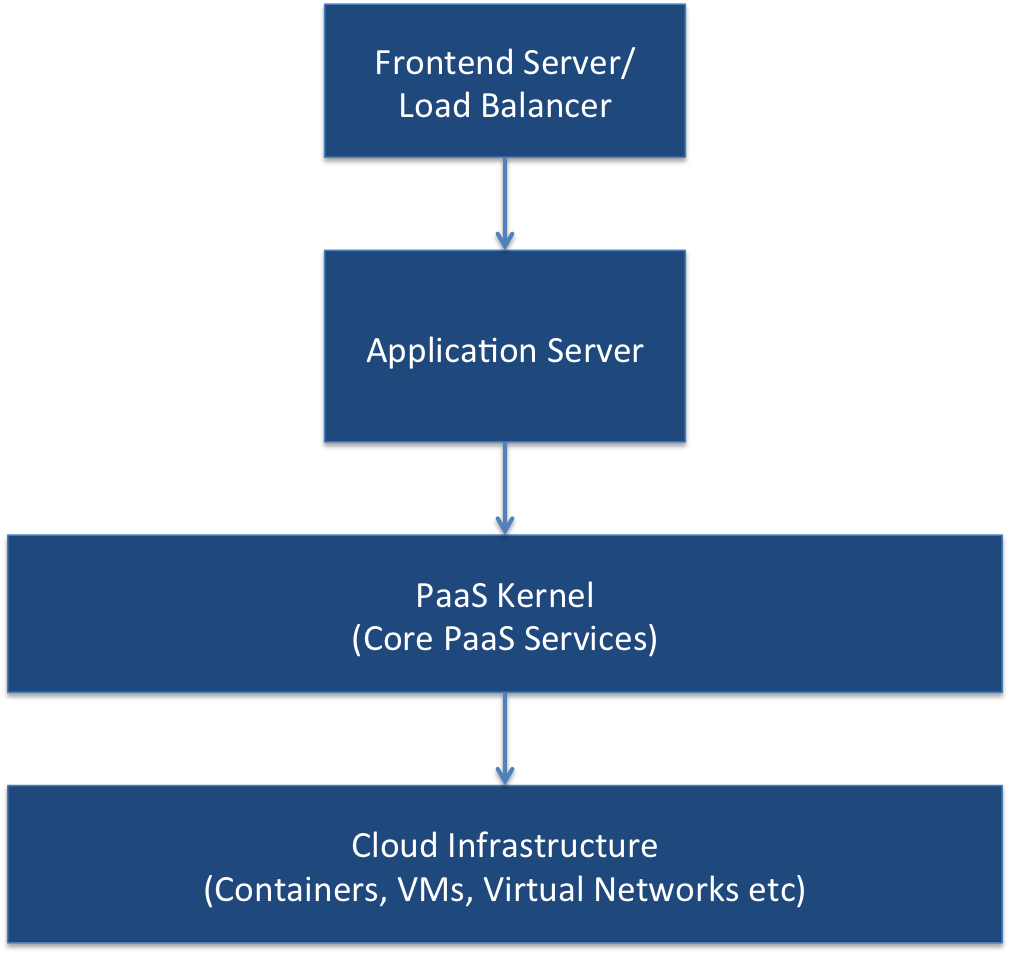
\includegraphics[scale=0.5]{paas_architecture}
\caption{PaaS system organization.}
\label{fig:paas_architecture}
\end{figure}

Figure~\ref{fig:paas_architecture} shows the key system layers of a typical PaaS cloud. Arrows indicate
the flow of data and control in response to application requests.

At the lowest level of a PaaS cloud is an infrastructure that consists of the necessary compute, storage
and networking resources. How this infrastructure is set up may vary from a simple cluster of physical 
machines to a comprehensive Infrastructure-as-a-Service (IaaS) solution. In large scale PaaS clouds,
this layer typically consists of many virtual machines and/or containers with the ability to acquire more
resources on the fly.

On top of the infrastructure layer lies the PaaS kernel. This is a collection of managed, scalable
services that high-level application developers can compose into their applications. The provided services
may include database services, caching services, queueing services and much more. Some PaaS clouds
provide a managed set of APIs (an SDK) for the application developer to access these fundamental services. 
In that case all interactions between the applications and the PaaS kernel must take place through
the cloud provider specified APIs (e.g. Google App Engine). 

One level above the PaaS kernel we find the application servers that are used to deploy and run
applications. Application servers provide the necessary integration (linkage) between application code and the
underlying PaaS kernel, while sandboxing application code for secure, multi-tenant operation. On top
of the application servers layer resides the fronted and load balancing layer. This layer is responsible
for receiving all application requests, filtering them and routing them to an appropriate application
server instance for further execution. As the fronted server, it is the entry point for PaaS-deployed
applications for all application clients.

\section{Cloud APM Architecture}
\subsection{Logical and Physical Layouts of the APM}
\begin{figure}
\centering
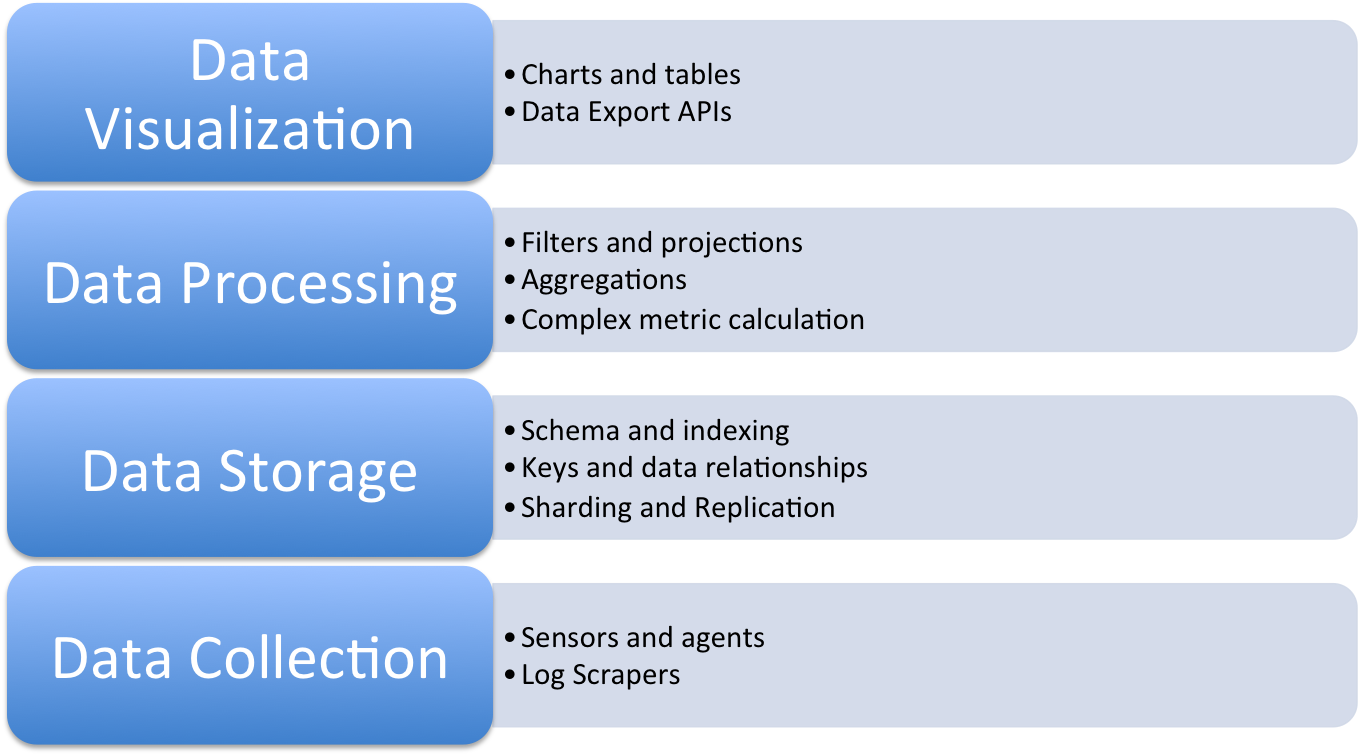
\includegraphics[scale=0.5]{apm_functions}
\caption{Key functions of the APM.}
\label{fig:apm_functions}
\end{figure}

\begin{figure}
\centering
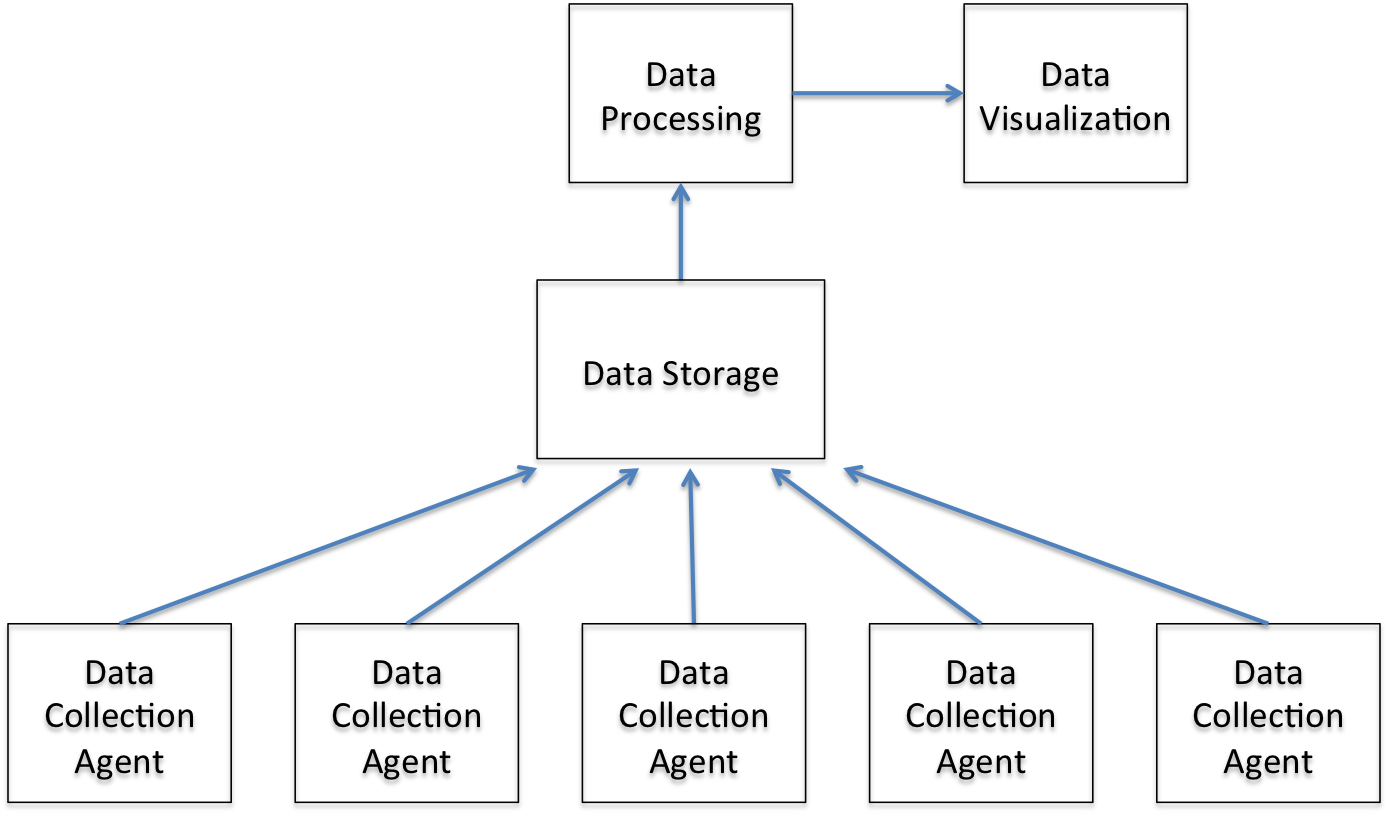
\includegraphics[scale=0.5]{apm_layout}
\caption{Physical view of the APM functions.}
\label{fig:apm_layout}
\end{figure}

Like most system monitoring solutions, the proposed cloud APM needs to serve four major functions: Data
collection, storage, processing (analytics) and visualization. Figure~\ref{fig:apm_functions} shows the
logical organization of these functions in the APM, and various tasks that fall under each of them.
Figure~\ref{fig:apm_layout} shows a physical deployment view of the said functions. Arrows indicate
the flow of information through the APM.

Data collection is performed by various sensors and agents that instrument the applications and the
core components of the PaaS cloud. While sensors are very primitive in their capability to monitor
a given component, an agent may intelligently adapt to changing conditions, making decisions on
what information to capture and how often. Instrumentations should be lightweight and as non-intrusive
as possible so their existence does not put any additional overhead on the applications.

Data storage components should be capable of
dealing with potentially very high volumes of data. The data needs to be organized and indexed
to facilitate efficient retrieval, and replicated to maintain reliability and high availability. 

Data processing components should also be capable of processing large volumes of data in near real-time,
while supporting a wide range of data analytics features such as filters, projections and aggregations. 
They will employ various statistical and perhaps even machine learning methods to understand the
data, detect anomalies and identify bottlenecks in the system.

Data visualization layer mainly consists of graphical interfaces (dashboards) for displaying various
metrics computed by the data processing components. Additionally it may also have APIs to export
the calculated results and trigger alerts. 

\subsection{APM Integration with the PaaS}
\end{document}